\subsection{Задача 1}

Воспользуемся критерием Баумана. Ясно, что для определения знаков всех крайних матриц достаточно найти наименьшее и наибольшее возможное значение точечного определителя матрицы $\mathbf{A}$:

\begin{equation}
\textrm{det} \mathbf{A} = (1 \pm \varepsilon) ^ 2 - (1.1 \pm \varepsilon)(1 \pm \varepsilon)
\end{equation}

Разность достигает \textbf{наибольшего} значения, когда уменьшаемое достигает \textbf{наибольшего} значения, а вычитаемое \textbf{наименьшего}.
	
\begin{equation} \label{maxdet}
\textrm{max det} \mathbf{A} = \varepsilon ^2 + 4.1 \varepsilon - 0.1
\end{equation}	

Разность достигает \textbf{наименьшего} значения, когда уменьшаемое достигает  \textbf{наименьшего} значения, а вычитаемое \textbf{наибольшего}.

\begin{equation}
\textrm{min det} \mathbf{A} = - 2 \varepsilon ^2 - 2.1 \varepsilon - 0.1
\end{equation}	

Видно, что минимум строго отрицательный, а значит, нам необходимо определить из \ref{maxdet}, при каких $\varepsilon$ наибольший определитель имеет отрицательное значение.

Решая квадратное уравнение, получаем:
\begin{equation}
	\varepsilon < \frac{-4.1 + \sqrt{4.1 ^ 2 + 0.4}}{2} \approx 0.024
\end{equation}

Итак, матрица особенна, когда $\varepsilon < 0.024$, следовательно, неособенна, когда $\varepsilon > 0.024$.

\subsection{Задача 2}
Решение данной задачи основывается на использовании признака Бекка совместно с бинарным поиском: примем сначала интервал неопределённости достаточно большим, чтобы $\mathbf{A}$ содержала особенные матрицы (скажем, скажем, $[0; 200]$). $\varepsilon$ (то есть текущее приближение его нижней границы) вычисляется как середина интервала неопределённости. Далее, если при текущем $\varepsilon$ результат применения признака Бекка отрицательный (то есть матрица неособенна), то сдвигаем правую границу поиска на текущий $\varepsilon$. Иначе сдвигаем левую. Вычисления производились с точностью до третьего знака после запятой. Результаты для разных размерностей матрицы приведены в следующей таблице:

\begin{table}[H]
	\begin{center}
		\begin{tabular}{|c|c|}
			\hline
			Размерность & $\varepsilon$ \\
			\hline
			2 & 1.000 \\
			\hline
			3 & 0.593 \\
			\hline
			4 & 0.419 \\
			\hline
			5 & 0.324 \\
			\hline
			6 & 0.262 \\
			\hline
		\end{tabular}
		\caption{Ответ ко второй задаче. Признак Бекка}
	\end{center}
\end{table}

\begin{figure}[H]
	\begin{center}
		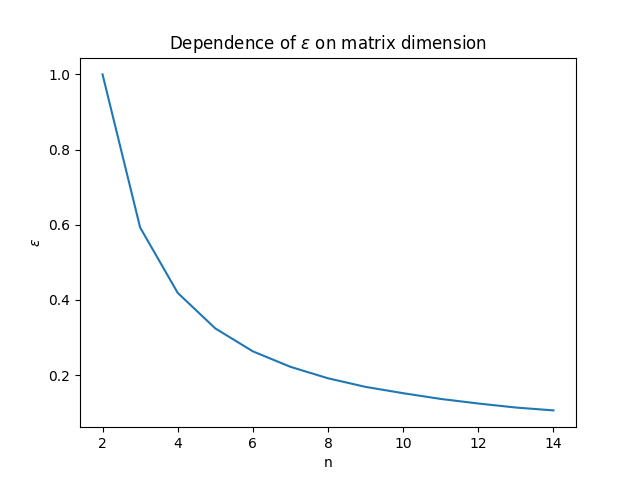
\includegraphics[scale=0.7]{degenmat}
		\label{pic:degenmat}
		\caption{Зависимость параметра $\varepsilon$ от размерности матрицы}
	\end{center}
\end{figure}

\begin{remark}
	Результаты следует интерпретировать как: ``При $\varepsilon$ б\'{о}льших, чем в таблице, матрица является особенной''.
\end{remark}